%!TEX root = ../thesis.tex

\section{Introduction}
\thispagestyle{plain}

\mypar{Rectangular layout}
  A  \emph{rectangular layout} (or simply \emph{layout}) $\L$ is a partition of a axis-parallel rectangle into a finite set of interior-disjoint axis-parallel rectangles. Hence the interior of this rectangle contains vertical and horizontal line segments. We will call any such line segment that is not extended any further on either side a \emph{maximal segment}. Such an layout is \emph{one-sided} if every maximal segment has only one rectangle on one of its sides and \emph{$k$-sided} if every maximal segment has at most $k$ rectangle on one of its sides.

  We say two layouts are  \emph{combinatorially equivalent} or simply \emph{equivalent} when their rectangles have the same adjacencies with the same orientation(horizontal or vertical) between their rectangles.

  Consider for example Figure \ref{fig:intr:segmentdefs}. The three highlighted lines are all line segments. However only the red and blue segment are maximal segments. The red segment is one-sided and the blue segment is $2$-sided. The whole layout is $2$-sided as well. The layout in Figure \ref{fig:intr:vertonesided} we have a $4$-sided layout.

  \begin{figure}
      \centering
      \begin{subfigure}[b]{0.45 \textwidth}
        \centering
        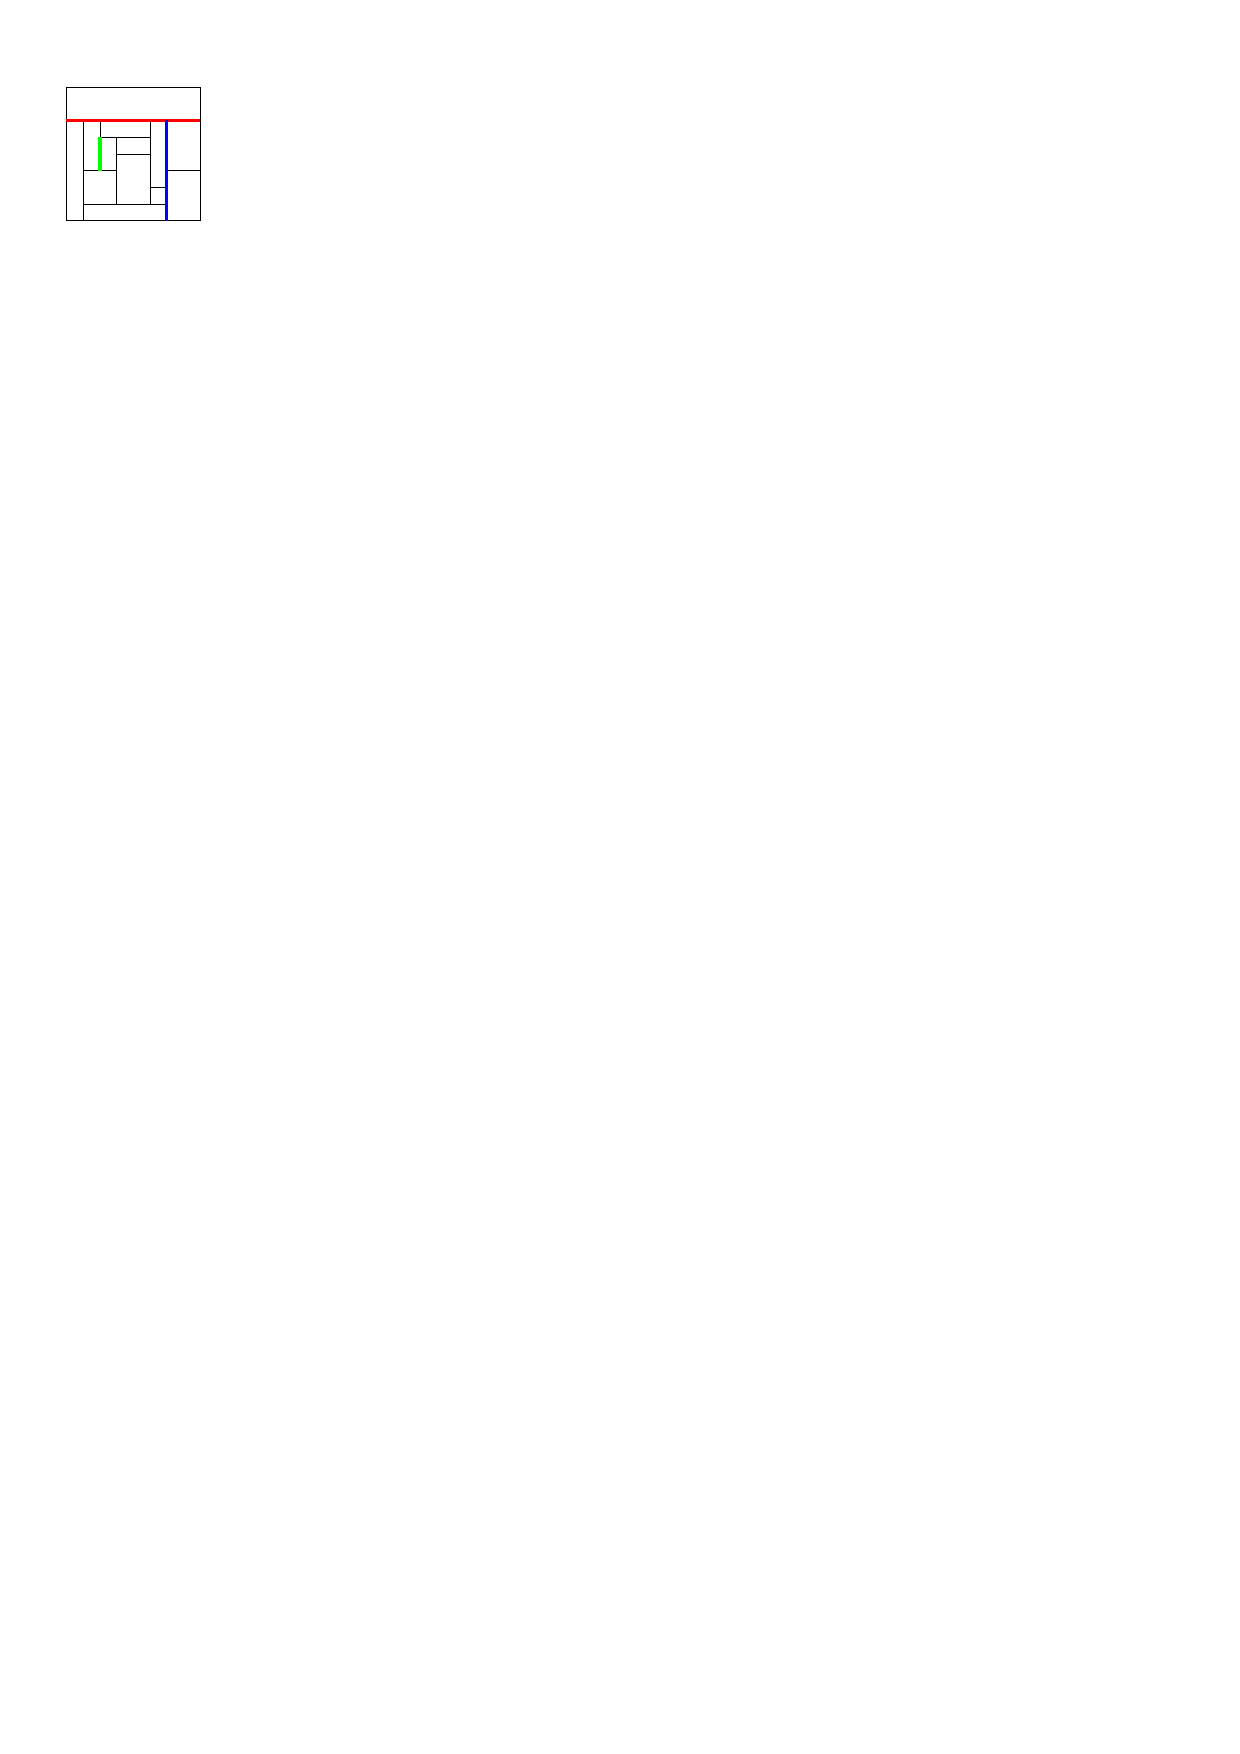
\includegraphics[scale=1]{rectangularDuals/img/segmentdefs}
        \caption{A rectangular layout}
        \label{fig:intr:segmentdefs}
      \end{subfigure}
      ~
      \begin{subfigure}[b]{0.45 \textwidth}
        \centering
        
\includegraphics[scale=1]{rectangularDuals/img/vertonesided}
        \caption{Another rectangular layout}
        \label{fig:intr:vertonesided}
      \end{subfigure}
      \caption{}
      \label{fig:intr:graphs}
  \end{figure}

\mypar{Graphs}
  A \emph{graph} $G$ is an abstraction for a network. The objects are represented by a set of \emph{vertices}. Connections are represented by \emph{edges}. Each edge connects two \emph{vertices}. In all graphs every pair of vertices is connected by at most one edge and there are no edges starting and ending at the same vertex. That is, all graphs are \emph{simple}. An edge is \emph{incident} to a vertex $v$ if that edge connects $v$ to another vertex. The \emph{degree} of a vertex is the number of edges incident to this vertex.
  All graphs in this thesis are \emph{planar}. That is, they can be embedded in the plane without their edges crossing. A \emph{face} is connected component of the maximal subset of the plane that is disjoint from the embedded graph. The \emph{degree} of a face is the number of vertices on its boundary. A \emph{triangular} face is a face of degree $3$. One and only one of the faces will be unbounded, we call this face the \emph{outer face}.
  A vertex is \emph{incident} to a face when it lies on its boundary.

  All graphs in this thesis will be \emph{triangulations of the $k$-gon}. They have a outer face of degree $k$ and interior faces of degree $3$.
  %Vertices bordering the outer face are \emph{outer vertices} while all other vertices are \emph{interior vertices}. Furthermore, the cycle formed by all vertices outer vertices is the \emph{outer cycle}.
  Triangulations of the $k$-gon are called \emph{(plane) triangulated graphs} by some authors.

\mypar{Rectangular duals}
  Two vertices are \emph{adjacent} when they are connected by an edge. Two rectangles are \emph{adjacent} when their boundaries overlap. A \emph{rectangular dual} of $G$ is a rectangular layout whose adjacencies are the same as those of $G$ for a bijection between vertices and rectangles.

\mypar{Corner assignments}
  If we want to consider which graphs do have a rectangular dual then we need to introduce the notion of a \emph{corner assignment}.
  A corner assignment $\ext G$ of $G$ is a augmentation of $G$ with $4$ vertices (which we call its \emph{poles}). Such that every interior face has degree $3$, the exterior face has degree $4$ and all poles are incident to the outer face

  A corner assignment of $G$ only exists if $G$ is a triangulation of the $k$-gon for some $k$. Otherwise there is no way of adding poles that makes all the interior faces of degree $3$. Which is why we only consider triangulations of the $k$-gon in this thesis. The corner assignment $\ext G$ is a triangulation of the $4$-gon. Each corner assignment fixes which of the rectangles are in the corners of the rectangular dual $\L$, which explains the terminology.


\mypar{Existance and uniqueness}
  Now we can answer the question which graphs admit a rectangular dual. The following result was shown independently by Kozminski and Kinnen \cite{Kozminski1984} and Ungar \cite{Ungar1953}
  \fxnote{Q Double citation. The inline ones should probably go but K and K and U becomes ambigious.}

  \begin{thrm}[Existence of a rectangular dual \cite{Kozminski1984, Ungar1953}]
    \label{th:rect:exsitenceREctangularDual}
    A triangulation of the $k$-gon $\G$ has a rectangular dual if and only if it has an corner assignment without separating triangles $\ext \G$
  \end{thrm}

  A graph $G$ can have multiple rectangular duals. $G$ can even have duals that are not equivalent. As an example one can consider the two non-equivalent duals of the same graph given in Figure \ref{fig:intr:graphs}.

\mypar{Rectangular cartograms}
  In for example atlases \emph{rectangular cartograms} are used to display information. A rectangular cartogram is a map where the regions are replaced by rectangles while keeping their adjacencies. The size of each region changes according to the variable displayed in the cartogram.  A rectangular cartogram is the rectangular dual of the adjacency graph of the map $G$.
  \fxnote{Figure of cartogram, where to find. Pres of speckman?}
  If the areas change it might be that a certain rectangular layout can not fulfill its adjacencies anymore and we have to switch to another non-equivalent rectangular dual of $G$.

  We would to find a rectangular dual that has adjacencies that hold regardless of the area sizes we assign to each rectangle. We say such a dual is \emph{area-universal}.
  Eppstein et al. have shown that rectangular duals are area-universal exactly when they are one-sided.~\cite{Eppstein2012} Unfortunately not all graphs admit a one-sided dual. One such graph is given by Rinsma.~\cite{Rinsma1987} \fxwarning{TODO figure of this graph with ciation}

\mypar{Results}
  Unfortunately $k$-sided layouts for $k>1$ are not area-universal but we suspect that for small $k$ they are more robust to changes in the areas of their rectangles. This thesis has two results on $k$-sidedness.
  \fxwarning{TODO Make this robust to changes notion more quative?  Explain why many sides are bad e.g. suing figure of many sided layout}
  \begin{enumerate}
    \item There is a family of graphs $G_k$ that for any $k \in \N$ has members that are not $k$-sided (Theorem \ref{fix:th:family}).
    \item Triangulations of the $k$-gon $G$ that have a corner assignment without separating 4-cycles are $d$-sided, where $d$ is the maximal degree of the vertices of $G$. (Theorem \ref{th:dsided})
  \end{enumerate}

\mypar{Overview}
\fxwarning[inline,nomargin]{TODO}
